\documentclass[oneside,12pt]{Classes/aesm_edspia}

\usepackage{minitoc}
\usepackage[latin1]{inputenc}
\usepackage[english,french]{babel}
\usepackage[T1]{fontenc}
\usepackage{amsmath}
\usepackage{lmodern}%font modern
\rmfamily
\DeclareFontShape{T1}{lmr}{bx}{sc}{<->ssub * cmr/bx/sc}{} 
\usepackage{lettrine}
\usepackage{tabularx}
\usepackage{epsfig, floatflt, amssymb} 
\usepackage{moreverb} %% pour le verbatim en boite
\usepackage{cases}%equations en systemes num�rot�s - soluce possible package : CASES
\usepackage{multirow} %% pour regrouper un texte sur plusieurs lignes dans une table
\usepackage{url} %% pour citer les url par \url
\usepackage[all]{xy} %% pour la barre au dessus des symboles
\usepackage{textcomp} %% pour le symbol pour mille par \textperthousand et degr�s par \degres
\usepackage[right]{eurosym}
\usepackage{setspace} %interligne simple, double etc...
\usepackage{Classes/eurosans} %%pour le symbole \euro
\usepackage{epic,eepic}
\usepackage{soul}
\usepackage[nottoc]{tocbibind} % tables des figures, des matieres et autres dans la TOC
\usepackage{fancybox}
\usepackage[leftcaption]{sidecap}
\usepackage[labelsep=endash, textfont={footnotesize, singlespacing}, margin=10pt, format=plain, labelfont=bf]{caption}
\usepackage[Conny]{Classes/fncychap} %en tete chapitrage
\newcommand{\ie}{c.-\`a-d.~}
\hbadness=10000% pb d'overfull box r�gl�
\hfuzz=50pt
\pdfcompresslevel9 % pour compresser le pdf final au maximum
\pdfoptionpdfminorversion=5 % pour accept� les images PDF version 1.5 (ex: celles produites par Office 2007)
\def\underscore{\char`\_}
\makeatletter
\renewcommand{\thesection}{\arabic {section}}
\renewcommand{\SC@figure@vpos}{c}% centrer verticalement le caption avec le package sidecap...
\renewcommand{\fnum@figure}{\small\textbf{Figure~\thefigure}}
\renewcommand{\fnum@table}{\small\textbf{Tableau~\thetable}}

\makeatother
\usepackage{subfig}
\def\thechapter{\Roman{chapter}}

%\usepackage[framed,numbered,autolinebreaks,useliterate]{Classes/mcode}


%%% Listings

\usepackage{listings}
\lstloadlanguages{xml, java}
	
	 \usepackage{listings}
  \usepackage{courier}
 \lstset{
         basicstyle=\footnotesize\ttfamily, 
         %numbers=left,               
         numberstyle=\tiny,          
         %stepnumber=2,               
         numbersep=5pt,              
         tabsize=2,                  
         extendedchars=true,         
         breaklines=true,            
         keywordstyle=\color[rgb]{0.43,0,0}\textbf,
    		frame=b,
         commentstyle=\color[rgb]{0.51,0.51,0.51} \textit ,
         stringstyle=\ttfamily  \color[rgb]{0,0.44,0} ,
         showspaces=false,           
         showtabs=false,             
         xleftmargin=17pt,
         framexleftmargin=17pt,
         framexrightmargin=5pt,
         framexbottommargin=4pt,
         %backgroundcolor=\color{lightgray},
         showstringspaces=false            
 }
 
 \usepackage{caption}
\DeclareCaptionFont{white}{\color{white}}
\DeclareCaptionFont{red}{\color{red}}
\DeclareCaptionFont{black}{\color{black}}
\DeclareCaptionFormat{listing}{\colorbox[cmyk]{0.43, 0.35, 0.35,0.01}{\parbox{\textwidth}{\hspace{15pt}#1#2#3}}}
\captionsetup[lstlisting]{format=listing,labelfont=black,textfont=white, singlelinecheck=false, margin=0pt, font={bf,footnotesize}}


%%%%%%%%%%%%%%%%%%%%%%%%%%%%%%%%%%%%%%%%%%%
\begin{document}
%%%%%%%%%%%%%%%%%%%%%%%%%%%%%%%%%%%%%%%%%%%
\renewcommand\figurename{\small\textbf{Figure}} 

\addtocounter{page}{-1}%pour revenir � 0

% Pour remplir la page de garde
\AuteurA{Anis} {BARKAOUI} 
%\AuteurB{Flen2} {FOULENI}
%\AuteurC{Flen3} {FOULENI} 
%\AuteurD{Flen4} {FOULENI}

\Encadrant{Mme}{Lilia}{SFAXI}
\EncadrantS{M.} {Charles} {LOOMIS}

\Filiere{G�nie Logiciel}
\datesout{--/--/2015}



\President{M. President} {FLEN}     %% Pr�sident du Jury
\RapporteurA{Mme. Rapporteur} {FLENA} %%Rapporteur



\AnneeUniv{2014/2015}

%%%%%%%%%%%%%%%%%%%%%%%%%%%%%%%%%%%%%%%%%%%
\makethese %% cr�e la couverture.

\onehalfspacing

% une page blanche (deuxi�me de couverture)
\newpage\thispagestyle{empty}\addtocounter{page}{-3}
\null\newpage\thispagestyle{empty}


\frontmatter %num�rotation en iii
\pagestyle{fancy}
\fancyhf{}
\fancyhead[R]{Remerciements}
\fancyfoot[R]{\thepage}
\renewcommand{\headrulewidth}{0.5pt}
\renewcommand{\footrulewidth}{0pt}

\chapter*{Remerciements}
%===================================================================

Nous tenons � exprimer notre sinc�re reconnaissance et notre profonde gratitude aux personnes suivantes qui ont aid� � la production de cet ouvrage :\\

� Monsieur \textbf{Charles LOOMIS}, Monsieur \textbf{Marc-Elian BEGIN} et Madame \textbf{Louise MERIFIELD}, les BigBoss de l'entreprise \textbf{SixSq}, pour la confiance qu'ils m'ont accord� afin de b�n�ficier de ce stage de fin d'�tudes.\\

� Monsieur \textbf{Charles LOOMIS}, mon encadrant au sein de l'�quipe de d�veloppement, pour l'int�r�t qu'il m'a transmis au sujet de la solution Big Data au sein de la plateforme SlipStream et pour la compr�hension globale relative � ce th�me que je suis parvenue � d�velopper tout au long de mon stage � \textbf{SixSq}.\\


� Madame \textbf{Lilia SFAXI}, mon tuteur de stage � l'Institut National des Sciences Appliqu�es et de Technologie, mod�le de douce patience, pour son merveilleux soutien scientifique, moral et amical, pour son patient travail de reconsolidation des acquis cognitifs et pour ses g�n�reux conseils concernant la pr�sentation de cet ouvrage.\\


� tout le cadre enseignant de l'\textbf{INSAT} et surtout mes professeurs qui par leur engagement scientifique et �ducatif, durant ces cinq ann�es d'�tudes, ont �t� pour moi une source d'inspiration.\\


Mes vifs remerciements s'adressent aux membres du jury, pour l'honneur qu'ils m'ont fait en examinant ce m�moire de fin d'�tudes, soyez assur�s de ma respectueuse consid�ration.


%%%%%%%% TOC

%profondeur dans la table des mati�res et de la num�rotation des sections

\setcounter{secnumdepth}{3}
\setcounter{tocdepth}{3}


\renewcommand{\contentsname}%
    {Table des Mati�res}%

%%%%minitoc
\dominitoc % g�n�re la minitoc
\nomtcrule % supprime les lignes horizontales de la minitoc
\renewcommand{\mtctitle}{Plan} % Modifie le titre de la minitoc

%%%%
\tableofcontents

\renewcommand{\headrulewidth}{0.5pt}
\renewcommand{\footrulewidth}{0pt}
\fancyhead[R]{Table des Mati�res}


%%%%%%%% Figures

\makeatletter
%\renewcommand{a\thefigure}{\@arabic\c@figure}
\@addtoreset{figure}{chapter}
\makeatother

\renewcommand{\headrulewidth}{0.5pt}
\renewcommand{\footrulewidth}{0pt}
\renewcommand\listfigurename{Liste des Figures}
\listoffigures \mtcaddchapter 

\fancyhead[R]{Liste des Figures}
\newpage


%%%%%%%% Tableaux

\makeatletter

\renewcommand{\headrulewidth}{0.5pt}
\renewcommand{\footrulewidth}{0pt}
\renewcommand\listtablename{Liste des Tableaux}

\listoftables  \mtcaddchapter 

\fancyhead[R]{Liste des Tableaux}

%%%%%%%%%%%%%%%%%%%%%%%%%%%%%%%%%%%
%\fancyhead[R]{R�sum�s}

\chapter*{R�sum�}
\addcontentsline{toc}{chapter}{R�sum�}
%===================================================================

Notre projet de fin d'�tudes consiste � r�aliser et mettre en place une solution Big Data au sein de la plateforme SlipStream. Principalement, il s'agit d'automatiser le processus de d�ploiement d'un cluster Hadoop dans un environnement de Cloud Computing. L'utilisateur final de notre projet peut d�ployer, en un seul clic, dans la plupart des Clouds existent sur le march� : un cluster Hadoop dont le nombre de noeuds au choix, des consoles d'administrations pour contr�ler et g�rer les servies de Hadoop et des autres outils pour connecter et utiliser les machines du cluster d�ploy�.

\chapter*{Abstract}
\addcontentsline{toc}{chapter}{Abstract}
%===================================================================

This is the english abstract of your project. It must be longer and presented in more details than the abstract you write on the back of your report.


%%%%%%%%%%%%%%%%%%%%%%%%%%%%%%%%%%%

                       
\mainmatter %num�ros arabes
\pagestyle{fancy}
\fancyhead[R]{Introduction G�n�rale}
\chapter*{Introduction G�n�rale}

\addcontentsline{toc}{chapter}{Introduction G�n�rale}
\begin{spacing}{1.2}
%==================================================================================================%

Pour �crire un bon rapport \cite{SFAXI2015} de projet en informatique, il existe certaines r�gles � respecter. Certes, chacun �crit son rapport avec sa propre plume et sa propre signature, mais certaines r�gles restent universelles    \cite{Latex}.\\

\textbf{La Table de mati�re} est la premi�re chose qu'un rapporteur va lire. Il faut qu'elle soit :
\begin{itemize}
\item Assez d�taill�e \footnote{Sans l'�tre trop}. En g�n�ral, 3 niveaux de num�ros suffisent;
\item Votre rapport doit �tre r�parti en chapitres �quilibr�s, � part l'introduction et la conclusion, naturellement plus courts que les autres;
\item Vos titres doivent �tre suffisamment personnalis�s pour donner une id�e sur votre travail. �viter le : � Conception �,  mais privil�gier : � Conception de l'application de gestion des $...$ � M�me s'ils vous paraissent longs, c'est mieux que 
d'avoir un sommaire impersonnel. \\
\end{itemize}

\textbf{Une introduction} doit �tre r�dig�e sous forme de paragraphes bien ficel�s. Elle est
normalement constitu�e de 4 grandes parties :
\begin{enumerate}
\item Le contexte de votre application : le domaine en g�n�ral, par exemple le domaine du web, de BI, des logiciels de gestion ?
\item La probl�matique : quels sont les besoins qui, dans ce contexte l�, n�cessitent la r�alisation de votre projet?
\item La contribution : expliquer assez bri�vement en quoi consiste votre application, sans entrer dans les d�tails de r�alisation. Ne pas oublier qu'une introduction est
 cens�e introduire le travail, pas le r�sumer; 
 \item La composition du rapport : les diff�rents chapitres et leur composition. Il n'est pas n�cessaire de num�roter ces parties, mais les mettre plut�t sous forme de paragraphes successifs bien li�s.
\end{enumerate}






\end{spacing}



\fancyhf{}
\fancyhead[R]{Introduction G�n�rale}
\fancyfoot[R]{\thepage}
\renewcommand{\headrulewidth}{0.5pt}
\renewcommand{\footrulewidth}{0pt}


\setcounter{mtc}{5} %indique le num�ro r�el du chapitre, pour la mini table des mati�res
\chapter{Pr�sentation et cadre du projet}
\minitoc  %insert la minitoc

\graphicspath{{Chapitre0/figures/}}
%==============================================================================
\pagestyle{fancy}
\fancyhf{}
\fancyhead[R]{\bfseries\rightmark}
\fancyfoot[R]{\thepage}
\renewcommand{\headrulewidth}{0.5pt}
\renewcommand{\footrulewidth}{0pt}
\renewcommand{\chaptermark}[1]{\markboth{\MakeUppercase{\chaptername~\thechapter. #1 }}{}}
\renewcommand{\sectionmark}[1]{\markright{\thechapter.\thesection~ #1}}

\begin{spacing}{1.2}
%==============================================================================

\section*{Introduction}
Une �tude th�orique \cite{YOUSFI2015} peut contenir l'une et/ou l'autre de ces deux parties :

TEST �����  TEST 

\section{Pr�sentation de l'entreprise 'SixSq'} 
SixSq est un leader europ\'{e}en dans le Cloud Computing qui fournit des solutions aux entreprises nationales et internationales de toutes tailles. L'entreprise se sp\'{e}cialise dans l'automatisation des processus, apportant des avantages financiers \`{a} ces clients via ces produits uniques: SlipStream\textregistered{} et NuvlaBox\textregistered{}. Son \'{e}quipe, qui se compose d'ing\'{e}nieurs de logiciels hautement qualifi\'{e}s, d\'{e}veloppeurs et administrateurs syst\`{e}me de 10 pays diff\'{e}rents, est bas\'{e} \`{a} Gen\`{e}ve, en Suisse.

\\Partenariats
\\SixSq collabore et participe \`{a} plusieurs programmes de partenariats. Et voici un r\'{e}sum\'{e} de certaines des relations  les plus importantes qu'elle~a~\'{e}tabli~: 
\\\textbf{EXOSCALE}: SixSq est le partenaire technologique d'Exoscale, le principal fournisseur de services de cloud suisse. Avec le connecteur SlipStream, les clients peuvent d\'{e}ployer leurs applications vers le cloud Exoscale en un seul clic.
\\\textbf{AMAZON}: SixSq est un fournisseur de solutions Amazon, avec un service de SlipStream d\'{e}di\'{e} et configur\'{e} pour d\'{e}ployer les applications sur le service EC2.  
\\\textbf{IBM}: SixSq est membre du programme \guillemotleft{}~IBM Partner World~\guillemotright{}. Elle a  certifi\'{e} SlipStream sur des solutions mat\'{e}rielles et  logicielles IBM. 
\\\textbf{Helix Nebula}: SixSq est un membre fondateur de la collaboration Helix Nebula, qui est un partenariat novateur entre les chercheurs scientifiques et les entreprises en Europe. 
\\\textbf{RHEA}~: SixSq forme un partenariat strat\'{e}gique avec RHEA, le premier fournisseur europ\'{e}en de services d'ing\'{e}nierie de syst\`{e}mes et de solutions logicielles pour les domaines~: l'a\'{e}rospatiale, la d\'{e}fense et  la s\'{e}curit\'{e} informatique.

\\Recherche et d\'{e}veloppement
\\SixSq est \`{a} la fronti\`{e}re entre le d\'{e}veloppement innovant et l'exploitation commerciale. SixSq est n\'{e} d'id\'{e}es cr\'{e}\'{e}es au CERN, l'organisation europ\'{e}enne pour la recherche nucl\'{e}aire. SixSq continue \`{a} participer \`{a} des projets de recherche et d\'{e}veloppement, \`{a} la fois aux niveaux national et international. 
\\\textbf{StratusLab} : est un logiciel de cloud IaaS (Infrastructure as a Service) issu d'un projet europ\'{e}en (FP7) et d\'{e}velopp\'{e} par une communaut\'{e} open-source.
\\\textbf{SCISSOR}  : con\c{c}oit un nouveau cadre de surveillance de la s\'{e}curit\'{e} SCADA de g\'{e}n\'{e}ration pour permettre, syst\`{e}mes connect\'{e}s, encore s\'{e}curis\'{e}s industriels contr\^{o}le. 
\\\textbf{PaaSword} : La S\'{e}curit\'{e} et la protection des donn\'{e}es sont  des obstacles importants \`{a} une large utilisation de plates-formes de cloud computing. PaaSword vise \`{a} r\'{e}duire ces obstacles en fournissant, le stockage s\'{e}curis\'{e} sur les services de cloud computing.
\\\textbf{CYCLONE} : d\'{e}veloppe une solution pour la gestion de la demande compl\`{e}te dynamique multi-cloud \`{a} partir de composants, de la production de qualit\'{e} existants. La solution comprend la gestion automatis\'{e}e de l'application, la mise en r\'{e}seau de pointe, une s\'{e}curit\'{e} de bout-en-bout, et de la gestion d'identit\'{e} f\'{e}d\'{e}r\'{e}e.  
\\\textbf{CELAR} : L'objectif du projet de CELAR est de d\'{e}velopper des m\'{e}thodes et des outils open-source pour l'application et le contr\^{o}le multi-grains, le provisionnement des ressources \'{e}lastique pour des applications de Cloud de mani\`{e}re automatis\'{e}e.

\\Clients et R\'{e}f\'{e}rences
\\Ces clients sont de grandes et petites int\'{e}grateurs de syst\`{e}mes, des soci\'{e}t\'{e}s de haute technologie, les institutions et les organisations internationales. Elle appr\'{e}cie des relations transparentes, fond\'{e}es sur la confiance et l'honn\^{e}tet\'{e}. Et Parmi ses clients on trouve:
\\\textbf{Atos} est une soci\'{e}t\'{e} internationale de services de technologie de l'information avec chiffre d'affaires 8,5 milliards d'euros en 2011 et 74 000 employeurs dans 42 pays.  Il est le partenaire informatique mondial des Jeux olympiques et paralympiques et est cot\'{e}e sur le march\'{e} Eurolist de Paris.
\\\textbf{Citrix Systems} ~est une~entreprise~multinationale~am\'{e}ricaine fond\'{e}e en 1989~qui propose des produits de collaboration, de virtualisation et de mise en r\'{e}seau pour faciliter le travail mobile et l'adoption des services cloud. Citrix compte plus de 330~000  entreprises clientes dans le monde entier.
\\\textbf{L'Union europ\'{e}enne de radio-t\'{e}l\'{e}vision}~est une organisation internationale cr\'{e}\'{e}e en 1950, la plus importante association professionnelle de radiodiffuseurs nationaux dans le monde avec 75 membres actifs dans 56 pays d'Europe, d'Afrique du Nord~et du~Proche-Orient.
\\\textbf{L'Agence spatiale europ\'{e}enne}, \'{e}galement d\'{e}sign\'{e}e sous on acronyme anglais ESA (European Space Agency), est une agence spatiale intergouvernementale coordonnant les projets spatiaux men\'{e}s en commun par une vingtaine de pays europ\'{e}ens. L'agence spatiale, qui par son budget 4 433 millions d'euros en 2015 est la troisi\`{e}me agence spatiale dans le monde apr\`{e}s la NASA et l'agence spatiale f\'{e}d\'{e}rale russe.
\\\textbf{Le~Centre europ\'{e}en des op\'{e}rations spatiales}~(en~anglais: ~European Space Operations Centre~:~ESOC), situ\'{e} \`{a}~Darmstadt~en Allemagne, est charg\'{e} du suivi de toutes les~sondes spatiales~qui sont sous le contr\^{o}le total de l'Agence spatiale europ\'{e}enne~(ESA).
\\\textbf{L'INFN} - l'Institut National de Physique Nucl\'{e}aire - est un institut d\'{e}di\'{e} \`{a} l'\'{e}tude des constituants fondamentaux de la mati\`{e}re, et m\`{e}ne des recherches th\'{e}oriques etexp\'{e}rimentales dans les domaines de subnucl\'{e}aire, nucl\'{e}aire et la physique des astroparticules.
\\\textbf{Interoute} est une~entreprise~de~t\'{e}l\'{e}communications~qui  poss\`{e}de le plus grand r\'{e}seau de nouvelle g\'{e}n\'{e}ration couvrant l'Union europ\'{e}enne, de Londres \`{a} Varsovie, de Stockholm \`{a} la Sicile et au-del\`{a}  dans les \'{e}conomies \'{e}mergentes du continent, y compris la Turquie, avec des stations d'atterrissage de dix sous-marins qui couvrent le pourtour de l'Europe. A l'Ouest, les liens r\'{e}seau \`{a} p\^{o}le majeur de t\'{e}l\'{e}communications en Am\'{e}rique du Nord. A l'Est, le r\'{e}seau relie l'Asie, \`{a} Hong Kong et au Moyen-Orient, via Duba\"{\i}, en Europe. Dans le Sud, l'Afrique, du Cap-town \`{a} Tunis se connecte directement \`{a} l'Europe par Interoute.
\\\textbf{Le Groupe SciSys} est un d\'{e}veloppeur de premier plan de services de TIC, e-Business et des solutions technologiques de pointe qui op\`{e}re dans un large \'{e}ventail de secteurs de march\'{e}, y compris l'espace, les services publics, de la d\'{e}fense, le gouvernement, la communication, les services aux entreprises, les m\'{e}dias et la diffusion et le transport.
\\\textbf{Thales Alenia Space}: leader europ\'{e}en des syst\`{e}mes satellitaires et acteur majeur des infrastructures orbitales, Thales Alenia Space est une joint-venture entre Thales et Finmeccanica et forme avec Telespazio une Alliance spatiale. Thales Alenia Space est une r\'{e}f\'{e}rence mondiale dans les t\'{e}l\'{e}communications, observation radar et optique de la Terre.
\\\textbf{Le CERN}, l'organisation europ\'{e}enne pour la recherche nucl\'{e}aire, est l'un des plus grands et des plus prestigieux laboratoires scientifiques du monde. Il a pour vocation la physique fondamentale, la d\'{e}couverte des constituants et des lois de l'Univers. Comment l'univers a-t-il commenc\'{e}? Les physiciens du CERN cherchent des r\'{e}ponses \`{a} cette question , en utilisant les acc\'{e}l\'{e}rateurs de particules les plus puissants.







\section{Cloud Computing et Big Data}
Le Cloud computing est un mod\`{e}le ~en \'{e}volution et ses d\'{e}finitions, cas d'usages, technologies, avantages et risques seront progressivement affin\'{e}es. L'industrie du Cloud Computing comporte un tr\`{e}s vaste \'{e}cosyst\`{e}me de mod\`{e}les, de fournisseurs et de march\'{e}s sp\'{e}cialis\'{e}s.~
Le Cloud Computing est un mod\`{e}le Informatique qui permet un acc\`{e}s facile et \`{a} la demande par le r\'{e}seau \`{a} un ensemble partag\'{e} de ressources informatiques configurables (serveurs, stockage, applications et services) qui peuvent \^{e}tre rapidement provisionn\'{e}es et lib\'{e}r\'{e}es par ~un minimum d'efforts de gestion ou d'interaction avec le fournisseur du service.
Le mod\`{e}le du Cloud Computing privil\'{e}gie la haute disponibilit\'{e}. Il se compose de~cinq ~caract\'{e}ristiques essentielles, de~trois mod\`{e}les de service~et de~quatre mod\`{e}les de d\'{e}ploiement.

\\
\\Les cinq caract\'{e}ristiques essentielles du Cloud computing
\\L'utilisation de ressources \`{a} distance n'est pas nouveau. Le \textquotedblleft{}time sharing\textquotedblright{} -utilisation partag\'{e}e d'un ordinateur en langage Basic- avait fait son apparition en 1966. On parlait alors de la \guillemotleft{}~prise de calcul~\guillemotright{} \`{a} c\^{o}t\'{e} de la prise de courant.. D\`{e}s le d\'{e}but des ann\'{e}es 70, les activit\'{e}s \textquotedblleft{}service bureau\textquotedblright{} ou \textquotedblleft{}traitement \`{a} fa\c{c}on\textquotedblright{} partageaient des traitements comme les payes ou les facturations sur des infrastructures communes avec souvent une facturation \`{a} l'usage. Plus r\'{e}cemment, sous le nom \textquotedblleft{}Outsourcing\textquotedblright{}, l'h\'{e}bergement et l'exploitation des applications des entreprises \`{a} distance se sont largement d\'{e}velopp\'{e}s. Ces activit\'{e}s n'avaient pas chang\'{e} l'architecture des syst\`{e}mes. Les gains provenaient d'une mise en commun de locaux et de moyens humains et techniques sp\'{e}cialis\'{e}s dans l'exploitation de syst\`{e}mes et d'applications ~existantes.
\\Le mod\`{e}le Cloud Computing se diff\'{e}rencie par les cinq caract\'{e}ristiques essentielles suivantes~:
\\\textbf{Acc\`{e}s aux services par l'utilisateur \`{a} la demande} : La mise en \oe{}uvre des syst\`{e}mes est enti\`{e}rement automatis\'{e}e et c'est l'utilisateur, au moyen d'une console de commande, qui met en place et g\`{e}re la configuration \`{a} distance.
\\\textbf{Acc\`{e}s r\'{e}seau large bande} : Ces centres de traitement sont g\'{e}n\'{e}ralement raccord\'{e}s directement sur le backbone Internet pour b\'{e}n\'{e}ficier d'une excellente connectivit\'{e}. Les grands fournisseurs r\'{e}partissent les centres de traitement sur la plan\`{e}te pour fournir un acc\`{e}s aux syst\`{e}mes en moins de 50 ms de n'importe quel endroit.
\\\textbf{R\'{e}servoir de ressources (non localis\'{e}es)} : La plupart de ces centres comportent des dizaines de milliers de serveurs et de moyens de stockage pour permettre des mont\'{e}es en charge rapides. Il est souvent possible de choisir une zone g\'{e}ographique pour mettre les donn\'{e}es \textquotedblleft{}pr\`{e}s\textquotedblright{} des utilisateurs.
\\\textbf{Redimensionnement rapide (\'{e}lasticit\'{e})} : La mise en ligne d'une nouvelle instance d'un serveur est r\'{e}alis\'{e}e en quelques minutes, l'arr\^{e}t et le red\'{e}marrage en quelques secondes. Toutes ces op\'{e}rations peuvent s'effectuer automatiquement par des scripts. Ces m\'{e}canismes de gestion permettent de b\'{e}n\'{e}ficier pleinement de la facturation \`{a} l'usage en adaptant la puissance de calcul au trafic instantan\'{e}.
\\\textbf{Facturation \`{a} l'usage} : Il n'y a g\'{e}n\'{e}ralement pas de co\^{u}t de mise en service (c'est l'utilisateur qui r\'{e}alise les op\'{e}rations). La facturation est calcul\'{e}e en fonction de la dur\'{e}e et de la quantit\'{e} de ressources utilis\'{e}es. Une unit\'{e} de traitement stopp\'{e}e n'est pas factur\'{e}e.


\\Les trois mod\`{e}les de services
\\Trois mod\`{e}les de services peuvent \^{e}tre offerts sur le Cloud :~Software as a Service~(SaaS),~Platform as a Service~(PaaS), ~Infrastructure as a Service~(IaaS).
Ces trois mod\`{e}les de service doivent \^{e}tre d\'{e}ploy\'{e}s sur des Infrastructures qui poss\`{e}dent les cinq caract\'{e}ristiques essentielles cit\'{e}es plus haut pour \^{e}tre consid\'{e}r\'{e}es comme du Cloud Computing.

\\\textbf{Software as a Service (SaaS)} : Ce mod\`{e}le de service est caract\'{e}ris\'{e}e par l'utilisation d'une application partag\'{e}e qui fonctionne sur une infrastructure Cloud. L'utilisateur acc\`{e}de ~\`{a} l'application par le r\'{e}seau au travers de divers types de terminaux (souvent via un navigateur web). L'administrateur de l'application ne g\`{e}re pas et ne contr\^{o}le pas l'infrastructure sous-jacente (r\'{e}seaux, serveurs, applications, stockage). Il ne contr\^{o}le pas les fonctions de l'application \`{a} l'exception d'un param\'{e}trage de quelques fonctions utilisateurs limit\'{e}es.

\\\textbf{Platform as a Service (PaaS)} : L'utilisateur a la possibilit\'{e} de cr\'{e}er et de d\'{e}ployer sur une infrastructure Cloud PaaS ses propres applications en utilisant les langages et les outils du fournisseur. .L'utilisateur ne g\`{e}re pas ou ne contr\^{o}le pas l'infrastructure Cloud sous-jacente (r\'{e}seaux, serveurs, stockage) mais l'utilisateur contr\^{o}le l'application d\'{e}ploy\'{e}e et sa configuration.


\\\textbf{Infrastructure as a Service (IaaS)} : L'utilisateur loue des moyens de calcul et de stockage, des capacit\'{e}s r\'{e}seau et d'autres ressources indispensables (partage de charge, pare-feu, cache). L'utilisateur a la possibilit\'{e} de d\'{e}ployer n'importe quel type de logiciel incluant les syst\`{e}mes d'exploitation.
L'utilisateur ne g\`{e}re pas ou ne contr\^{o}le pas l'infrastructure Cloud sous-jacente mais il a le contr\^{o}le sur les syst\`{e}mes d'exploitation, le stockage et les applications. Il peut aussi choisir les caract\'{e}ristiques principales des \'{e}quipements r\'{e}seau comme le partage de charge, les pare-feu, etc.

\\
\\\textbf{Les quatre mod\`{e}les de d\'{e}ploiement}
\\Certains distinguent quatre mod\`{e}les de d\'{e}ploiement. Nous les citons ci-apr\`{e}s bien que ces mod\`{e}les n'aient que peu ~d'influence sur les caract\'{e}ristiques techniques des syst\`{e}mes d\'{e}ploy\'{e}es.



\\\textbf{Cloud priv\'{e}}
L'infrastructure Cloud est utilis\'{e}e par une seule organisation. Elle peut \^{e}tre g\'{e}r\'{e}e par l'organisation ou par une tierce partie. L'infrastructure peut \^{e}tre plac\'{e}e dans les locaux de l'organisation ou \`{a} l'ext\'{e}rieur

\\\textbf{Cloud communautaire}
L'infrastructure Cloud est partag\'{e}e par plusieurs organisations pour les besoins d'une communaut\'{e} qui souhaite mettre en commun des moyens (s\'{e}curit\'{e}, conformit\'{e}, etc..). Elle peut \^{e}tre g\'{e}r\'{e}e par les organisations ou par une tierce partie et peut \^{e}tre plac\'{e}e ~dans les locaux ou \`{a} l'ext\'{e}rieur.

\\\textbf{Cloud public}
L'infrastructure cloud est ouverte au public ou \`{a} de grands groupes industriels. Cette infrastructure est poss\'{e}d\'{e}e par une organisation qui vend des services Cloud. C'est le cas le plus courant. C'est celui de la plate-forme Amazon Web Services d\'{e}j\`{a} cit\'{e}e.

\\\textbf{Cloud hybride}
L'infrastructure Cloud est compos\'{e}e d'un ou plusieurs mod\`{e}les ~ci-dessus qui restent des entit\'{e}s s\'{e}par\'{e}es. Ces infrastructures sont li\'{e}es entre elles par la m\^{e}me technologie qui autorise la portabilit\'{e} des applications et des donn\'{e}es. ~C'est une excellente solution pour r\'{e}partir ses moyens en fonction des avantages recherch\'{e}s.


\\\textbf{Les caract\'{e}ristiques communes des diff\'{e}rents mod\`{e}les de Cloud}
\\Le Cloud computing tire parti d'un certain nombre de caract\'{e}ristiques pour fournir des services dans des conditions techniques et \'{e}conomiques tr\`{e}s avantageuses. C'est un peu comme la production d'\'{e}lectricit\'{e}. La plupart des entreprises et des particuliers ont int\'{e}r\^{e}t \`{a} utiliser des fournisseurs dont c'est le m\'{e}tier pour garantir la fiabilit\'{e} et les meilleures conditions \'{e}conomiques. Parmi ces caract\'{e}ristiques communes, on trouve g\'{e}n\'{e}ralement~:

\\\textbf{Des infrastructures gigantesques}
\\Par exemple, le syst\`{e}me de stockage en ligne~Amazon S3~est pass\'{e} de 14 milliards d'objets en janvier 2008 \`{a} 905 milliards d'objets en mars~ 2012 ce qui entra\^{\i}ne des prix de plus en plus bas : de l'ordre de 0.1 euro par giga-octets et par mois.

\\\textbf{Une grande homog\'{e}n\'{e}it\'{e} des moyens}
\\Les syst\`{e}mes regroupent des milliers de composants identiques ce qui simplifie la gestion, la fiabilit\'{e}, ~l'audit et la s\'{e}curit\'{e}.

\\\textbf{virtualisation}
\\La virtualisation est une caract\'{e}ristique indispensable qui pr\'{e}sente de tr\`{e}s nombreux avantages. Le mat\'{e}riel est remplac\'{e} par du logiciel avec tous les avantages du logiciel~: cr\'{e}er une nouvelle machine ou sauvegarder son \'{e}tat consiste \`{a} copier un fichier d'o\`{u} un \'{e}norme gain de temps et d'argent. La machine virtuelle ne tombe pratiquement jamais en panne ce qui accroit s\'{e}rieusement la fiabilit\'{e} des syst\`{e}mes. On peut continuer \`{a} utiliser des machines qui ne sont plus fabriqu\'{e}es. Le pourcentage d'utilisation r\'{e}elle d'un serveur physique d\'{e}passe rarement 15\%. Sur la m\^{e}me puissance de calcul on peut faire fonctionner plusieurs serveurs. Lorsqu'une configuration est utilis\'{e}e pour des d\'{e}veloppements, des op\'{e}rations de recette ou des tests de charge, il est possible de lib\'{e}rer des ressources en archivant la configuration. La remise en ligne du syst\`{e}me lorsque c'est n\'{e}cessaire se fait en quelques minutes.

\\\textbf{Elasticit\'{e} }
\\L'ensemble des caract\'{e}ristiques pr\'{e}c\'{e}dentes (taille, homog\'{e}n\'{e}it\'{e} et virtualisation) permet d'adapter automatiquement la capacit\'{e} de traitement d'une application \`{a} la demande constat\'{e}e. La mise en ligne d'un nouveau serveur peut s'effectuer en moins d'une minute. Il n'est plus n\'{e}cessaire de s'\'{e}quiper pour absorber des pointes de trafic.


\\\textbf{Co\^{u}ts de logiciels tr\`{e}s r\'{e}duits}
\\La plupart des plates-formes publiques utilisent des logiciels open source gratuits. Les co\^{u}ts des logiciels propri\'{e}taires sont souvent factur\'{e}s \`{a} l'usage sans n\'{e}cessiter l'achat de licences. La plupart de ces logiciels sont d\'{e}j\`{a} pr\'{e}install\'{e}s et pr\'{e}configur\'{e}s ce qui fait gagner beaucoup de temps comme expliqu\'{e} dans l'exemple d'utilisation du dernier chapitre.


\\\textbf{Distribution g\'{e}ographique}
\\Les grandes plates-formes publiques disposent de centres r\'{e}partis sur la plan\`{e}te pour r\'{e}duire les risques et placer les donn\'{e}es au plus pr\`{e}s des utilisateurs.


\\\textbf{Orientation Service}
\\Les fonctions fournies aux utilisateurs se pr\'{e}sentent sous la forme de~Web services (REST)~faciles \`{a} utiliser dans un navigateur ou mieux par des scripts automatis\'{e}s. Des groupes de standardisation se sont cr\'{e}\'{e}s pour d\'{e}finir des interfaces communes et simplifier ainsi le passage d'une infrastructure \`{a} une autre.


\\\textbf{Fonctions de s\'{e}curit\'{e} avanc\'{e}es}
\\la s\'{e}curit\'{e} est une pr\'{e}occupation majeure des organisations qui utilisent les services du Cloud. Ces plates-formes disposent g\'{e}n\'{e}ralement de nombreux syst\`{e}mes de protection, hors de port\'{e}e des moyens de la plupart des organisations.














\section{M�thodologie de travail} 
On va pr�senter la m�thodologie Scrum + Une comparison avec les autres m�thodologies + Outlis utilis�s


\section*{Conclusion}
La conclusion est en g�n�ral sans num�rotation, et n'appara�t pas dans la table des mati�res.


%==============================================================================
\end{spacing}

\setcounter{mtc}{5} %indique le num�ro r�el du chapitre, pour la mini table des mati�res
\chapter{Contexte G�n�ral Et Cadre Du Projet}
\minitoc  %insert la minitoc

\graphicspath{{Chapitre1/figures/}}
%==============================================================================
\pagestyle{fancy}
\fancyhf{}
\fancyhead[R]{\bfseries\rightmark}
\fancyfoot[R]{\thepage}
\renewcommand{\headrulewidth}{0.5pt}
\renewcommand{\footrulewidth}{0pt}
\renewcommand{\chaptermark}[1]{\markboth{\MakeUppercase{\chaptername~\thechapter. #1 }}{}}
\renewcommand{\sectionmark}[1]{\markright{\thechapter.\thesection~ #1}}

\begin{spacing}{1.2}
%==============================================================================

\section*{Introduction}
L'objectif de ce premier chapitre consiste � mettre notre projet dans le contexte g�n�ral o� il �volue. Ainsi � une premi�re �tape, nous commen�ons par pr�senter l'entreprise d'accueil. Ensuite, nous d�crivons bri�vement le contexte du projet et la probl�matique � r�soudre. Enfin, nous pr�sentons les m�thodologies du travail adopt�es et la planification du projet.



\section{Pr�sentation de l'entreprise SixSq} 
\subsection{Pr�sentation g�n�rale}
SixSq est un leader europ�en dans le Cloud Computing qui fournit des solutions aux entreprises nationales et internationales de toutes tailles. L'entreprise se sp�cialise dans l'automatisation des processus, apportant des avantages financiers � ces clients via ces produits uniques: SlipStream� et NuvlaBox�. Son �quipe, qui se compose d'ing�nieurs de logiciels hautement qualifi�s, d�veloppeurs et administrateurs syst�me de 10 pays diff�rents, est bas�e � Gen�ve, en Suisse.

\begin{figure}[H]
\centering

\includegraphics[scale=0.47]{SixSq_logo.png}
\caption{Logo de l'entreprise SixSq}
\label{fig:fig1}
\end{figure}


\subsection{Partenariats}

SixSq collabore et participe � plusieurs programmes de partenariats. Et voici un r�sum� de certaines des relations les plus importantes qu'elle a �tabli :

\begin{description}
\item[EXOSCALE] SixSq est le partenaire technologique d'Exoscale, le principal fournisseur de services de Cloud suisse.

\item[AMAZON] SixSq est un fournisseur de solutions Amazon, avec un service de SlipStream d�di� et configur� pour d�ployer les applications sur le service EC2.

\item[IBM] SixSq est membre du programme � IBM Partner World �. Elle a certifi� SlipStream sur des solutions mat�rielles et logicielles IBM. 

\item[Helix Nebula] SixSq est un membre fondateur de la collaboration Helix Nebula, qui est un partenariat novateur entre les chercheurs scientifiques et les entreprises en Europe.

\item[RHEA] SixSq forme un partenariat strat�gique avec RHEA, le premier fournisseur europ�en de solutions logicielles pour les domaines : l'a�rospatiale, la d�fense et la s�curit� informatique.
\end{description}



\subsection{Recherche et D�veloppement}
SixSq est � la fronti�re entre le d�veloppement innovant et l'exploitation commerciale. SixSq est n�e d'id�es cr��es au CERN, le centre europ�en pour la recherche nucl�aire. SixSq continue � participer � des projets de recherche et d�veloppement, � la fois aux niveaux national et international tel que: H2020, StratusLab, SCISSOR, PAChA, PaaSword, CYCLONE, CELAR.



\subsection{Clients et R�f�rences}
Ces clients sont de grandes et petites int�grateurs de syst�mes, des soci�t�s de haute technologie, les institutions et les organisations internationales. Elle appr�cie des relations transparentes, fond�es sur la confiance et l'honn�tet�. Parmi ses clients, nous citons :


\begin{description}

\item[Atos] est une soci�t� internationale de services de technologie de l'information avec chiffre d'affaires 8,5 milliards d'euros en 2011 et 74 000 employeurs dans 42 pays.

\item[Citrix Systems] est une entreprise multinationale am�ricaine fond�e en 1989 qui compte plus de 330 000 entreprises clientes dans le monde entier.

\item[L'Union europ�enne de radio-t�l�vision] est a plus importante association professionnelle de radiodiffuseurs nationaux dans le monde avec 75 membres actifs dans 56 pays.

\item[L'Agence spatiale europ�enne] (ESA: European Space Agency) est la troisi�me agence spatiale dans le monde apr�s la NASA et l'agence spatiale f�d�rale russe.


\item[Le Centre Europ�en des Op�rations Spatiales] est charg� du suivi de toutes les sondes spatiales qui sont sous le contr�le total de l'Agence spatiale europ�enne (ESA).

\item[L'Institut National de Physique Nucl�aire] est un institut d�di� � l'�tude des constituants fondamentaux de la mati�re.

\item[Interoute] est une entreprise de t�l�communications qui poss�de le plus grand r�seau de nouvelle g�n�ration couvrant l'Union europ�enne.


\item[Thales Alenia Space] est un leader europ�en des syst�mes satellitaires et une r�f�rence mondiale dans les t�l�communications, observation radar et optique de la Terre.

\item[Le Centre Europ�en pour la Recherche Nucl�aire (CERN)] est l'un des plus grands et des plus prestigieux laboratoires scientifiques du monde.

\end{description}




\section{Contexte et Probl�matique} 
Le Cloud Computing et les Big Data deviennent aujourd'hui une r�alit� pour la plupart des entreprises. Les professionnels ne se contentent plus de savoir comment stocker les Big Data, mais tentent d'analyser ces donn�es de fa�on pertinente pour r�pondre � des besoins m�tier r�els. Alors que le Cloud Computing poursuit son �volution, de plus en plus d'entreprises cr�ent des environnements Cloud efficaces et agiles, tandis que les fournisseurs �toffent leurs offres de services.\\


Dans ce contexte, il est donc logique que les DSI consid�rent le Cloud Computing comme une structure permettant de soutenir leurs projets de Big Data. Les outils qui traitent les vastes volumes de Big Data aux formats vari�s requi�rent des clusters de serveurs. Les Clouds sont d�j� d�ploy�s sur des pools de ressources (serveurs, �quipements de stockage et r�seau) �volutives selon les besoins. Le Cloud Computing offre un moyen rentable pour exploiter les technologies Big Data.\\


D'une part, les donn�es sont de plus en plus pr�cieuses. Aujourd'hui, la question n'est plus � quelles donn�es devons-nous stocker ? �, mais � que pouvons-nous faire avec ces donn�es ? �. Les entreprises cherchent � lib�rer toute la valeur potentielle de leurs donn�es afin d'en tirer des avantages concurrentiels. Le volume des donn�es d'entreprise s'est accru de 800 \% entre 2011 et 2015, avec 80 \% de donn�es non structur�es (e-mails, documents, vid�os, images, contenus des plateformes de r�seaux sociaux, etc.) et 20 \% de donn�es structur�es (transactions par carte de cr�dit, coordonn�es, etc.). \\


D'autre part, le Cloud Computing devient aujourd'hui une r�alit� pour de nombreuses entreprises, avec en particulier une forte pouss�e du d�ploiement des Clouds priv�s. La technologie Cloud atteint son niveau de maturit�, les obstacles � son adoption �tant progressivement �limin�s au fil des am�liorations en mati�re de s�curit� et d'int�gration des donn�es. De leur c�t�, les entreprises informatiques �voluent et s'adaptent pour prendre en charge les services Cloud. On assiste donc � un renforcement croissant de la confiance des entreprises envers les mod�les de distribution Cloud. \\

Les entreprises stockent et traitent de plus en plus de donn�es dans les environnements de Cloud Computing, constituant ce faisant d'immenses et pr�cieuses mines d'informations. Les architectures Cloud constituent en outre pour les utilisateurs m�tier des ressources �volutives, capables de s'adapter � leurs besoins. L'association entre des serveurs et syst�mes de stockage avec des outils de traitement Big Data tels que le logiciel Apache Hadoop fournit la puissance de calcul requise pour analyser de grandes quantit�s de donn�es de mani�re efficace et rentable. Mais le d�ploiement de ce type de logiciel dans un environnement de Cloud Computing repr�sente l'un des plus grands d�fis pour ses utilisateurs puisqu'il n�cessite une longue installation de plusieurs outils sur plusieurs machines virtuelles ainsi qu'une configuration tr�s complexe, ce qui augmente le risque d'erreur.\\

Dans ce contexte, notre mission consiste � r�aliser et mettre en place une solution Big Data au sien d'une plateforme multi-cloud afin d'automatiser le d�ploiement (l'installation et la configuration) d'une distribution Hadoop dans un environnement de Cloud Computing.


\section{M�thodologies adopt�es} 


\subsection{Le processus de d�veloppement � Scrum �}


\subsubsection{Choix m�thodologique}

Le choix du processus de d�veloppement est une �tape cruciale dans l'�laboration d'un projet. En effet, le processus de d�veloppement est constitu� d'une succession de phases allant de la sp�cification des besoins � la r�alisation et la livraison du produit.\\

Le choix d'une d�marche pour le processus de d�veloppement est li� � l'ampleur du projet, � l'�quipe qui le prendra en charge ainsi qu'� sa dur�e et aux moyens mis en oeuvre.\\

Alors, apr�s avoir parcouru les diff�rentes d�marches utilis�es en gestion de projets et en ayant connaissance de la dur�e limite'e de notre projet de fin d'
�tudes, nous avons opt� pour suivre La m�thodologie � Scrum � d'Agile.


\subsubsection{M�thodologie agile}

Une m�thodologie agile est une approche it�rative et incr�mentale pour le d�veloppement de logiciel, r�alis�e de mani�re tr�s collaborative par des �quipes responsabilis�es, en appliquant un c�r�monial minimal, qui produisent, dans un d�lai contraint, un logiciel de grande qualit� qui vise � r�pondre aux besoins changeants des utilisateurs.\\

Le but d'une m�thodologie agile est de maximiser la valeur ajout�e. Le d�veloppement s'effectuent par it�rations successives, il est possible, � la fin de chaque it�ration, de changer les priorit�s en faisant en sorte que les �l�ments apportant le plus de valeur soient r�alis�s a priori.\\

Les douze principes du manifeste agile sont : 
\begin{itemize}
\item Satisfaire le client en livrant t�t et r�guli�rement des logiciels utiles, qui offrent une v�ritable valeur ajout�e.
\item Accepter les changements, m�me tard dans le d�veloppement.
\item Livrer fr�quemment une application qui fonctionne.
\item Collaborer quotidiennement entre clients et d�veloppeurs.
\item B�tir le projet autour de personnes motiv�es en leur fournissant environnement et support, et en leur faisant confiance.
\item Communiquer par des conversations en face � face.
\item Mesurer la progression avec le logiciel qui fonctionne.
\item Garder un rythme de travail durable.
\item Rechercher l'excellence technique et la qualit� de la conception.
\item Laisser l'�quipe s'auto-organiser.
\item Rechercher la simplicit�.
\item � intervalles r�guliers, r�fl�chir aux moyens de devenir plus efficace.
\end{itemize}


\subsubsection{M�thodologie Scrum}

La m�thodologie Scrum est une m�thodologie agile dont le nom est un terme emprunt� au rugby qui signifie � la m�l�e �. Elle s'appuie sur le d�coupage des projets en it�rations encore nomm�es � sprints �. Un sprint peut avoir une dur�e qui varie g�n�ralement entre deux semaines et un mois.\\

Avant chaque sprint, les t�ches sont estim�es en temps et en complexit� � l'aide de certaines pratiques comme le � planning poker �, une mani�re ludique de chiffrer la complexit� des t�ches ou �volutions � l'aide de cartes � l'instar du c�l�bre jeu dont le nom est repris. Ces estimations permettent � la fois de planifier les livraisons, mais aussi d'estimer le co�t de ces t�ches aupr�s du client. Les fonctionnalit�s qui font l'objet d'un sprint constituent ce que l'on appelle un � sprint backlog � du produit �ventuellement livrable � la fin du sprint. Il est n�cessaire de distinguer le sprint backlog du � product backlog � qui lui correspond � l'ensemble des fonctionnalit�s attendues pour le produit sur l'ensemble des sprints.\\

La figure \ref{fig:fig2}  pr�sente le tableau de bord du dernier sprint de notre projet. �Waffle.io� est l'outil qui nous fournit ce tableau de bord afin d'appliquer la m�thodologie Scrum.\\
\begin{figure}[H]\centering
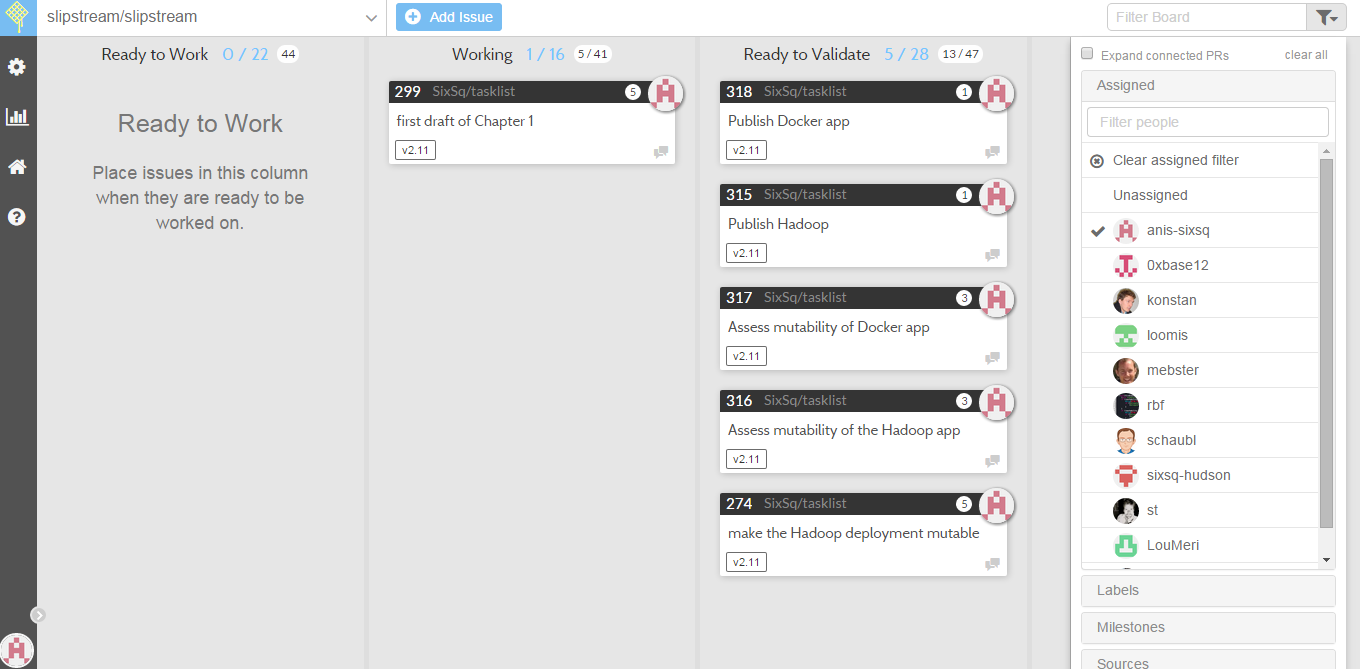
\includegraphics[scale=0.47]{waffle.png}
\caption{Tableau de bord du dernier sprint}
\label{fig:fig2}
\end{figure}




La m�thodologie Scrum est aussi caract�ris�e par une � m�l�e � quotidienne, encore appel�e � stand-up �, dans laquelle les collaborateurs (chefs de projets, d�veloppeurs et responsables fonctionnels) indiquent tour � tour les t�ches qu'ils ont effectu�es la veille, les difficult�s rencontr�es et enfin ce sur quoi ils vont poursuivre leur travail le jour suivant. Cela permet d'�valuer l'avancement du projet, de mobiliser des ressources l� o� cela est le plus n�cessaire, mais aussi de venir en aide aux collaborateurs rencontrant des difficult�s lorsque celles-ci ont d�j� �t� rencontr�es auparavant par d'autres membres de l'�quipe.\\

La figure \ref{fig:fig3} repr�sente le processus de la r�alisation d'un projet en utilisant la m�thodologie Scrum.\\
\begin{figure}[H]
\centering
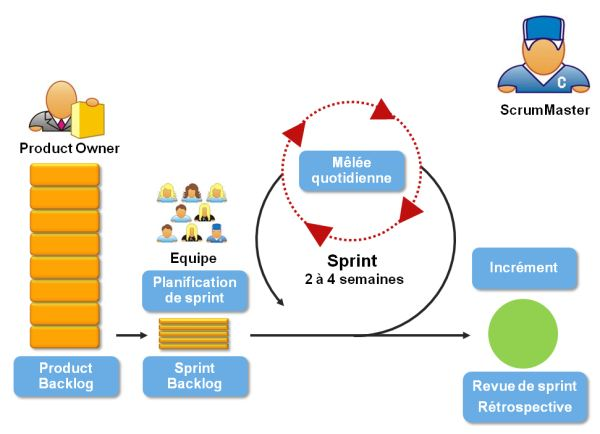
\includegraphics[scale=0.7]{methode-scrum.jpg}
\caption{Processus de la m�thodologie Scrum}
\label{fig:fig3}
\end{figure}


La m�thodologie Scrum d�finit trois r�les pour un projet.
\begin{enumerate}
\item Le product owner : il s'agit du repr�sentant officiel du client au sein d'un projet Scrum. Il est l'interlocuteur principal du Scrum Master et des membres de l'�quipe. Il d�finit les besoins du produit et r�dige les sp�cifications. Il peut se faire aider de responsables fonctionnels pour la r�daction des sp�cifications. Il est �galement charg� de d�finir et prioriser les users stories pour chaque sprint.
\item Le scrum master : il s'agit d'une personne charg�e de veiller � la mise en application de la m�thode et au respect de ses objectifs. Il ne s'agit pas d'un chef de projet, mais d'une personne charg�e de lever les obstacles �ventuels qui emp�cherait l'avancement de l'�quipe et du projet pendant les diff�rents sprints.
\item L'�quipe (� team members �) : ce sont les personnes charg�es de la r�alisation du sprint et d'un produit utilisable en fin de sprint. Il peut s'agir de d�veloppeurs, architectes, personnes charg�es de faire des tests fonctionnels...
\end{enumerate}




\subsection{Formalisme de mod�lisation � UML �}
Nous utilisons � Unified Modeling Language (UML) � pour la sp�cification et la conception de ce travail, ce langage est la base de plusieurs m�thodes Agile comme les processus unifi�s. UML permet de d�crire les besoins et documenter les syst�mes ainsi que d'esquisser les architectures logicielles. Il s'articule autour de neuf diagrammes d�di�s � la pr�sentation d'un concept particulier du syst�me �tudi�. Toutefois, pour �viter de surcharger le rapport et d'entrer dans certains d�tails techniques, nous ne pr�sentons que quelques diagrammes que nous jugeons utiles pour comprendre le projet, � savoir les diagrammes des cas d'utilisation et les diagrammes de s�quences :
\begin{itemize}
\item Les diagrammes de cas d'utilisation: permettent l'�num�ration des fonctions de l'application du point de vue de l'utilisateur.
\item Les diagrammes de s�quences: permettent une repr�sentation temporelle et comportementale des objets et leurs interactions.
\end{itemize}




\section{Planification du projet} 
Le projet s'est d�roul� pendant une dur�e de quatre mois et s'est �tendu sur la p�riode entre le 02 Mars 2015 et le 30 juin 2015. La figure \ref{fig:fig4}  illustre le plan suivi, repr�sentant les �tapes majeures � franchir afin d'aboutir � une solution fonctionnelle r�pondant aux crit�res d�finis par le cahier des charges.
\begin{figure}[H]
\centering
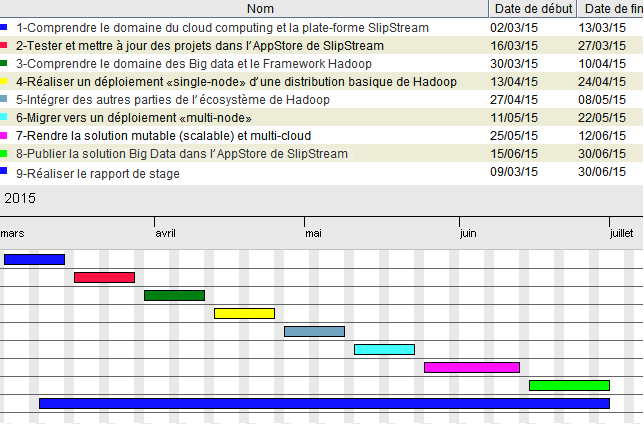
\includegraphics[scale=0.9]{gantt-1.png}
\caption{Planification du projet}
\label{fig:fig4}
\end{figure}


\section*{Conclusion}
Tout au long de ce chapitre, nous avons commenc� par la pr�sentation de l'entreprise SixSq, le contexte et la probl�matique de notre projet. Par suite, nous avons pr�sent� les m�thodologies adopt�es ainsi que la planification du projet. Dans le chapitre suivant, nous d�taillons les diff�rents domaines du travail ainsi que l'�tat de l'art .


%==============================================================================
\end{spacing}

\setcounter{chapter}{2}
\chapter{Conception de la solution Big Data au sein de SlipStream}
\minitoc %insert la minitoc
\graphicspath{{Chapitre2/figures/}}

%\DoPToC

%==============================================================================
\pagestyle{fancy}
\fancyhf{}
\fancyhead[R]{\bfseries\rightmark}
\fancyfoot[R]{\thepage}
\renewcommand{\headrulewidth}{0.5pt}
\renewcommand{\footrulewidth}{0pt}
\renewcommand{\chaptermark}[1]{\markboth{\MakeUppercase{\chaptername~\thechapter. #1 }}{}}
\renewcommand{\sectionmark}[1]{\markright{\thechapter.\thesection~ #1}}

\begin{spacing}{1.2}
%==============================================================================
\section*{Introduction} 
motivation de l'application (valorisation)

\section{Besoins fonctionnels}


\section{Diagrammes}
on va pr�senter les digrammes : usecase + sequence  //a discuter !!!

\section{Architecture}

 
\section*{Conclusion}
Faire ici une petite r�capitulation du chapitre, ainsi qu'une introduction du chapitre suivant.





%==============================================================================
\end{spacing}

\setcounter{mtc}{7}
\chapter{Analyse Et Sp�cification Des Besoins}
\minitoc %insert la minitoc
\graphicspath{{Chapitre3/figures/}}

%\DoPToC

%==============================================================================
\pagestyle{fancy}
\fancyhf{}
\fancyhead[R]{\bfseries\rightmark}
\fancyfoot[R]{\thepage}
\renewcommand{\headrulewidth}{0.5pt}
\renewcommand{\footrulewidth}{0pt}
\renewcommand{\chaptermark}[1]{\markboth{\MakeUppercase{\chaptername~\thechapter. #1 }}{}}
\renewcommand{\sectionmark}[1]{\markright{\thechapter.\thesection~ #1}}

\begin{spacing}{1.2}
%==============================================================================
\section*{Introduction} 
Ce chapitre contient une description compl�te du comportement du syst�me � d�velopper. Ce dernier pr�sente une analyse et une sp�cification des diff�rents besoins fonctionnels et non fonctionnels. Nous identifions, dans une premi�re partie, les acteurs du syst�me. Dans une deuxi�me partie, nous it�rons les exigences fonctionnelles et non fonctionnelles. Ensuite, nous analysons les besoins � travers l'�laboration des diagrammes de cas d'utilisation et de s�quence syst�me qui d�crivent toutes les interactions possibles entre les utilisateurs et la solution en termes de fonctionnalit�s.




\section{Identification des acteurs du syst�me}
Les acteurs �voqu�s dans le syst�me sont :

\begin{itemize}
\item  L'utilisateur de Hadoop :
\begin{itemize}
\item Est un simple utilisateur qui a un compte SlipStream.
\item Il doit �tre un client au moins d'un seul fournisseur Cloud (IaaS).
\item Il a le droit de d�ployer notre solution Hadoop dans une infrastructure Cloud.
\item Il a le droit d'utiliser et g�rer la solution Hadoop d�ploy�e.
\item Il a le droit de terminer la solution Hadoop d�ploy�e.
\end{itemize} 


\item L'administrateur de la solution Hadoop :
\begin{itemize}
\item Est un utilisateur SlipStream qui a le droit d'�diter la solution.
\item Il a le droit de voir et modifier la configuration des VMs de la solution.
\item II a le droit de mettre � jour la solution.
\end{itemize} 
\end{itemize} 





\section{Sp�cification des besoins}
La sp�cification des besoins met en relief les fonctionnalit�s utiles que doit fournir le syst�me. La solution � r�aliser doit satisfaire les besoins fonctionnels et non fonctionnels �num�r�s dans les deux prochaines sections.




\subsection{Besoins fonctionnels}
Nous d�taillons dans cette partie les principales fonctionnalit�s, que le syst�me doit fournir aux diff�rents acteurs, qui se pr�sentent comme suit:

\begin{itemize}
\item  \textbf{Utilisateur de Hadoop} La solution doit permettre aux utilisateurs:
\begin{itemize}
\item \textbf{Le d�ploiement d'un cluster Hadoop} : le syst�me doit permettre aux utilisateurs de d�ployer, en un seul clic, un cluster Hadoop dans un ou plusieurs Clouds au choix.
\item \textbf{L'utilisation des machines de Hadoop} : une fois Hadoop d�ploy�, le syst�me doit permettre aux utilisateurs de connecter � la machine �master� en mode SSH ou en mode graphique et utiliser tous les fonctionnalit�s de Hadoop � 2.x �.
\item \textbf{La gestion des services de Hadoop} : une fois Hadoop d�ploy�, le syst�me doit permettre aux utilisateurs de g�rer les diff�rents services de Hadoop.
\item \textbf{La gestion du cluster Hadoop} : une fois Hadoop d�ploy�, le syst�me doit permettre aux utilisateurs d'ajouter ou de terminer des machines �slaves� du cluster selon le besoin.
\item \textbf{La gestion des VMs du cluster} : une fois Hadoop d�ploy�, le syst�me doit permettre aux utilisateurs de g�rer les caract�ristiques des machines virtuelles utilis�es dans le d�ploiement.
\end{itemize} 



\item \textbf{Administrateur de la solution Hadoop}  La solution doit permettre � l'administrateur:
\begin{itemize}
\item \textbf{La mise � jour de la solution} : le syst�me doit permettre � l'administrateur de mettre � jour la version de Hadoop et les autres outils utilis�s dans la solution.
\item \textbf{La gestion des machines pr�configur�es de Hadoop} : le syst�me doit permettre � l'administrateur de g�rer les types d'instances et les images ID des VMs du cluster.
\item \textbf{La gestion de la s�curit� au niveau de Cloud} : le syst�me doit permettre � l'administrateur de g�rer le groupe de s�curit�.\\
\end{itemize} 
\end{itemize} 


\textbf{Remarque}:\\
Dans la suite de ce chapitre, nous ne d�taillerons que les cas d'utilisation de l'acteur � Utilisateur de Hadoop � puisque tout le travail � r�aliser est li� directement � cet acteur. Pour l'acteur � administrateur �, c'est la plateforme SlipStream qui g�re tous ces cas d'utilisation.\\





\subsection{Besoins non fonctionnels}
Notre objectif dans ce projet est de d�velopper une solution performante. Etant donn� qu'une application uniquement fonctionnelle et op�rationnelle ne garantit ni la satisfaction ni la fid�lit� des utilisateurs, nous devons prendre en consid�ration des crit�res non fonctionnels lors de la conception et l'impl�mentation de notre solution. Parmi ces exigences, nous citons:

\begin{itemize}
\item \textbf{Le temps de d�ploiement} : la solution doit permettre � l'utilisateur de d�ployer un cluster Hadoop dans un temps tr�s r�duit par rapport un d�ploiement manuel.
\item \textbf{L'ergonomie} : pendant le temps de d�ploiement, la solution doit afficher � l'utilisateur toutes les informations qui concernent l'�tat de d�ploiement. Apr�s la fin de d�ploiement, la solution doit fournir � l'utilisateur toutes les informations n�cessaires pour utiliser le cluster Hadoop d�ploy�.
\item \textbf{La performance des machines} : la solution doit permettre � l'utilisateur de d�ployer un cluster Hadoop performant qui r�pond � ses besoins en puissance de calcul.
\item \textbf{La s�curit�} : l'application doit respecter certaines r�gles relatives � la s�curit� des syst�mes informatiques. En effet, la solution g�n�re d'une mani�re al�atoire des mots de passe complexes pour permettre � l'utilisateur de s'authentifier au niveau des VMs et les interfaces d'administration.
\item \textbf{La maintenance} : les diff�rentes parties de la solution doivent �tre faciles � maintenir. Par cons�quent, le code doit �tre lisible, bien comment� et bien structur�.
\end{itemize} 





\section{Sp�cification d�taill�e des besoins}
Cette partie a pour objectif de d�crire le comportement attendu de l'application pour l'acteur � Utilisateur de Hadoop �. Pour cela nous nous basons sur les diagrammes de cas d'utilisation et de s�quence afin de mod�liser les diff�rentes fonctionnalit�s de notre solution.


\subsection{Cas d'utilisation de l'acteur � Utilisateur de Hadoop �}
Les diagrammes de cas d'utilisation permettent de recenser les grandes fonctionnalit�s de notre syst�me. Ainsi, dans cette partie, nous allons pr�senter le diagramme des cas d'utilisation pour l'acteur 'utilisateur de Hadoop'. Le diagramme dans la figure \ref{fig:fig3-1} pr�sente ces cas d'utilisation.
\begin{figure}[H]\centering
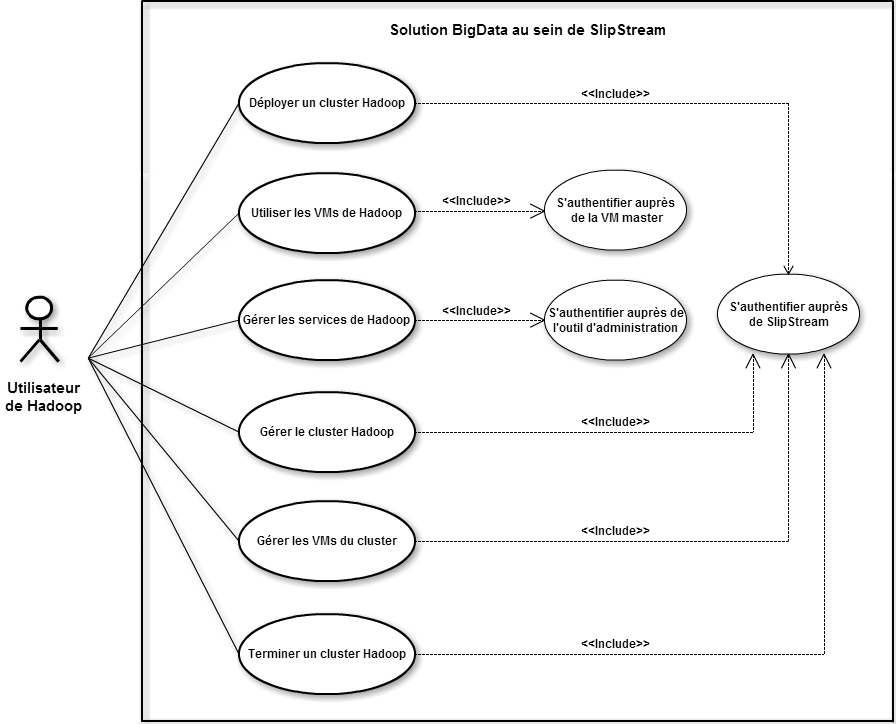
\includegraphics[scale=0.49]{Use-Case.png}
\caption{Diagramme de cas d'utilisation}
\label{fig:fig3-1}
\end{figure}


Dans cette partie, chaque cas d'utilisation fera l'objet d'une description d�taill�e illustrant son but, les diff�rentes possibilit�s de son d�roulement, les conditions n�cessaires � sa r�alisation, etc.

\subsubsection{Cas d'utilisation 'D�ployer un cluster Hadoop'}
Le but de cas d'utilisation 'D�ployer un cluster Hadoop' est le d�ploiement d'un cluster Hadoop en un seul clic � partir de l'AppStore de SlipStream dans un ou plusieurs Clouds. Ce cas d'utilisation montre que notre solution est une solution multi-cloud. Le tableau Tab \ref{tab:usecase-1}   ci-dessous illustre ce sc�nario.

\begin{table}[H]
	\centering
	\caption{D�roulement du sc�nario 'D�ployer un cluster Hadoop'}
	\footnotesize
	\begin{tabularx}{\linewidth}{|>{\bfseries \vspace*{\fill}}X ||>{\vspace*{\fill}}X<{\centering{}}|}	
			\hline 
			Titre & \bfseries Utilisateur: d�ployer un cluster Hadoop\\
			\hline \hline
			Intervenant		&	Utilisateur de Hadoop	\\
			\hline
			Pr�-condition	&	\begin{itemize}\item L'authentification aupr�s de SlipStream est  effectu�e avec succ�s.\item Le profil de l'utilisateur est bien configur�.\end{itemize}	\\
			
			\hline
			sc�narios		&	\begin{enumerate}\item L'utilisateur acc�de � l'AppStore de SlipStream.\item L'utilisateur clic sur le bouton 'Deploy' de Hadoop.\item Le syst�me affiche une fen�tre des param�tres de d�ploiement.\item L'utilisateur coche les options de d�ploiement au choix.\item L'utilisateur choisit le (ou les) Cloud(s) � utiliser.\item L'utilisateur choisit le nombre de VMs du cluster (master et slaves).\item L'utilisateur clic sur le bouton � Run deployment'.\item Le syst�me affiche la page de d�ploiement.\end{enumerate}	\\
			\hline
			Post-condition		&	Le syst�me lance l'automatisation du d�ploiement et affiche tous ses �tats (les actions, la progression...).	\\
			\hline
			Alternative(s)		&	Param�tres erron�s ou manquants.	\\
			
			\hline
	\end{tabularx}
	\label{tab:usecase-1}
\end{table}








\subsubsection{Cas d'utilisation 'Utiliser les VMs de Hadoop'}
Le but de cas d'utilisation 'Utiliser les VMs de Hadoop' est la connexion � la machine virtuelle 'Master' en mode SSH (en utilisant l'invite de commandes) ou en mode graphique (en utilisant un client VNC). Une fois l'utilisateur connect�, il utilise son cluster Hadoop. Le tableau Tab \ref{tab:usecase-2}   ci-dessous illustre ce sc�nario.\\

\begin{table}[H]
	\centering
	\caption{D�roulement du sc�nario 'Utiliser les VMs de Hadoop'}
	\footnotesize
	\begin{tabularx}{\linewidth}{|>{\bfseries \vspace*{\fill}}X ||>{\vspace*{\fill}}X<{\centering{}}|}	
			\hline 
			Titre & \bfseries Utilisateur: Utiliser les VMs de Hadoop\\
			\hline \hline
			Intervenant		&	Utilisateur de Hadoop	\\
			\hline
			Pr�-condition	&	Le d�ploiement est effectu� avec succ�s. \\
			\hline
			sc�narios		&	\begin{itemize}
			
			\item L'utilisateur connecte en mode SSH: 
			\begin{enumerate}
			\item Le syst�me fournit un lien de connexion SSH � la machine master de Hadoop. 
			\item L'utilisateur clic sur ce lien et connecte directement � cette machine.
			\end{enumerate}
			
			\item L'utilisateur connecte en mode graphique:
			\begin{enumerate}
			\item Le syst�me fournit un login et un mot de passe pour l'authentification aupr�s de la machine master.
			\item Le syst�me fournit une interface graphique de la machine master.
			\item L'utilisateur s'authentifie aupr�s de cette machine avec le couple (login et mot de passe) fourni.
			\item L'utilisateur utilise cette machine.
			\end{enumerate}
			
			\end{itemize}	\\
			\hline
			Post-condition		&	L'utilisateur profite de tous les services de Hadoop en mode Cloud.	\\
			\hline
			Alternative(s)		&	Login ou mot de passe erron�.	\\
			
			\hline
	\end{tabularx}
	\label{tab:usecase-2}
\end{table}


\newpage



\subsubsection{Cas d'utilisation 'G�rer les services de Hadoop'}
Le but de cas d'utilisation 'G�rer les services de Hadoop' est l'administration de tous les services de Hadoop d�ploy�s. Une fois le d�ploiement de Hadoop termin�, notre solution offre une interface graphique en mode SaaS qui permettre � l'utilisateur de g�rer, contr�ler, visualiser, ajouter, supprimer ... les services de Hadoop. Le tableau Tab \ref{tab:usecase-3} ci-dessous illustre ce sc�nario.\\

\begin{table}[H]
	\centering
	\caption{D�roulement du sc�nario 'G�rer les services de Hadoop'}
	\footnotesize
	\begin{tabularx}{\linewidth}{|>{\bfseries \vspace*{\fill}}X ||>{\vspace*{\fill}}X<{\centering{}}|}	
			\hline 
			Titre & \bfseries Utilisateur: G�rer les services de Hadoop\\
			\hline \hline
			Intervenant		&	Utilisateur de Hadoop	\\
			\hline
			Pr�-condition	&	Le d�ploiement est effectu� avec succ�s.	\\
			
			\hline
			sc�narios		&	\begin{enumerate}\item Le syst�me fournit un login et un mot de passe pour l'authentification aupr�s de l'outil d'administration en mode SaaS.\item Le syst�me fournit le lien pour connecter � cet outil.\item L'utilisateur clic sur ce lien et s'authentifie.\item L'utilisateur connecte � l'interface d'administration.\item L'utilisateur g�re et contr�le tous les services.\end{enumerate}	\\
			\hline
			Post-condition		&	Le syst�me applique toutes les actions lancer par l'utilisateur � partir de l'interface d'administration.\\
			\hline
			Alternative(s)		&	Ports ferm�s au niveau de fournisseur Cloud (IaaS).	\\
			
			\hline
	\end{tabularx}
	\label{tab:usecase-3}
\end{table}




\newpage





\subsubsection{Cas d'utilisation 'G�rer le cluster Hadoop'}
Le but de cas d'utilisation 'G�rer le cluster Hadoop' est de rendre le cluster d�ploy� scalable horizontalement. Selon les besoins des utilisateurs, notre solution offre la possibilit� d'ajouter ou de supprimer des VMs � slaves� du cluster. Ce cas d'utilisation montre l'�lasticit� notre solution ce qui est une caract�ristique fondamentale du Cloud Computing. Le tableau Tab \ref{tab:usecase-4} ci-dessous illustre ce sc�nario.\\

\begin{table}[H]
	\centering
	\caption{D�roulement du sc�nario 'G�rer le cluster Hadoop'}
	\footnotesize
	\begin{tabularx}{\linewidth}{|>{\bfseries \vspace*{\fill}}X ||>{\vspace*{\fill}}X<{\centering{}}|}	
			\hline 
			Titre & \bfseries Utilisateur: G�rer le cluster Hadoop\\
			\hline \hline
			Intervenant		&	Utilisateur de Hadoop	\\
			\hline
			Pr�-condition	&	\begin{itemize} \item Le d�ploiement est effectu� avec succ�s. \item SlipStream client est install� sur la machine d'utilisateur. \end{itemize}	\\
			
			\hline
			sc�narios		&	\begin{enumerate}\item L'utilisateur ex�cute les commandes SlipStream sp�cifi�es pour ajouter/terminer des VMs 'slaves' du cluster.\item Le syst�me r�affiche la page de d�ploiement avec la nouvelle configuration.\item L'utilisateur r�utilise son cluster.\end{enumerate}	\\
			\hline
			Post-condition		&	Le syst�me d�ploie/termine ces VMs et reconfigure toutes les VMs du cluster et l'outil d'administration.\\
			\hline
			Alternative(s)		&	\begin{itemize} \item Commandes erron�es.\item Non-respect du nombre minimal des VMs.\end{itemize}	\\
			
			\hline
	\end{tabularx}
	\label{tab:usecase-4}
\end{table}






\newpage


\subsubsection{Cas d'utilisation 'G�rer les VMs du cluster'}
Le but de cas d'utilisation 'G�rer les VMs du cluster' est de rendre chaque machine virtuelle du cluster scalable verticalement. Selon les besoins des utilisateurs, notre solution offre la possibilit� de modifier les caract�ristiques des VMs d�ploy�es en termes de CPU, RAM et DISC. Ce cas d'utilisation montre un autre type d'�lasticit� de notre solution. Le tableau Tab \ref{tab:usecase-5} ci-dessous illustre ce sc�nario.\\

\begin{table}[H]
	\centering
	\caption{D�roulement du sc�nario 'G�rer les VMs du cluster'}
	\footnotesize
	\begin{tabularx}{\linewidth}{|>{\bfseries \vspace*{\fill}}X ||>{\vspace*{\fill}}X<{\centering{}}|}	
			\hline 
			Titre & \bfseries Utilisateur: G�rer les VMs du cluster \\
			\hline \hline
			Intervenant		&	Utilisateur de Hadoop	\\
			\hline
			Pr�-condition	&	\begin{itemize} \item Le d�ploiement est effectu� avec succ�s. \item SlipStream client est install� sur la machine d'utilisateur. \end{itemize}	\\
			
			\hline
			sc�narios		&	\begin{enumerate}\item L'utilisateur ex�cute les commandes SlipStream sp�cifi�es pour modifier les caract�ristiques des VMs (CPU, RAM et DISC).\item Le syst�me r�affiche la page de d�ploiement.\item L'utilisateur r�utilise son cluster avec la nouvelle configuration des VMs.\end{enumerate}	\\
			\hline
			Post-condition		&	Le syst�me modifie les caract�ristiques de ces VMs et r�initialise l'outil d'administration.\\
			\hline
			Alternative(s)		&	\begin{itemize} \item Commandes erron�es.\item Non-respect des limites des ressources.\end{itemize}	\\
			
			\hline
	\end{tabularx}
	\label{tab:usecase-5}
\end{table}



\newpage


\subsubsection{Cas d'utilisation 'Terminer un cluster Hadoop'}
Le but de cas d'utilisation 'Terminer un cluster Hadoop' est de terminer tout un cluster d�ploy�. Une fois l'utilisateur finalis� son travail avec le cluster Hadoop, il peut le terminer en un seul clic � partir de SlipStream. Le tableau Tab \ref{tab:usecase-6} ci-dessous illustre ce sc�nario.\\

\begin{table}[H]
	\centering
	\caption{D�roulement du sc�nario 'Terminer un cluster Hadoop'}
	\footnotesize
	\begin{tabularx}{\linewidth}{|>{\bfseries \vspace*{\fill}}X ||>{\vspace*{\fill}}X<{\centering{}}|}	
			\hline 
			Titre & \bfseries Utilisateur: Terminer un cluster Hadoop \\
			\hline \hline
			Intervenant		&	Utilisateur de Hadoop	\\
			\hline
			Pr�-condition	&	\begin{itemize} \item L'authentification aupr�s de SlipStream est effectu�e avec succ�s.. \item Le d�ploiement du cluster est effectu�. \end{itemize}	\\
			
			\hline
			sc�narios		&	\begin{enumerate}\item L'utilisateur acc�de � la page du d�ploiement.\item L'utilisateur clic sur le bouton 'Terminate' du d�ploiement.\item Le syst�me affiche une fen�tre de confirmation.\item L'utilisateur clic sur le bouton 'Terminate'.\item Le syst�me r�affiche la page du d�ploiement avec l'�tat 'Terminated'.\end{enumerate}	\\
			\hline
			Post-condition		&	Le syst�me lance une requ�te vers le(s) Cloud(s) pour terminer toutes les VMs du cluster.\\
			\hline
			Alternative(s)		&		\\
			
			\hline
	\end{tabularx}
	\label{tab:usecase-6}
\end{table}











\newpage
\subsection{Interactions acteur-syst�me}
Les diagrammes de s�quences syst�me sont la repr�sentation graphique des interactions entre les acteurs et le syst�me selon un ordre chronologique dans la formation. Dans ce qui suit nous d�crivons les cas d'utilisation 'D�ployer un cluster Hadoop' et 'G�rer les services de Hadoop' gr�ce � des diagrammes de s�quence syst�me qui montrent les interactions entre les utilisateurs de Hadoop et le syst�me d'une mani�re globale.


\subsubsection{Cas d'utilisation 'D�ployer un cluster Hadoop'}
Les utilisateurs peuvent d�ployer un cluster Hadoop � partir de l'AppStore de SlipStream dans un ou plusieurs Clouds. Ce sc�nario est illustr� dans le diagramme de la  figure \ref{fig:fig3-2} .
\begin{figure}[H]\centering
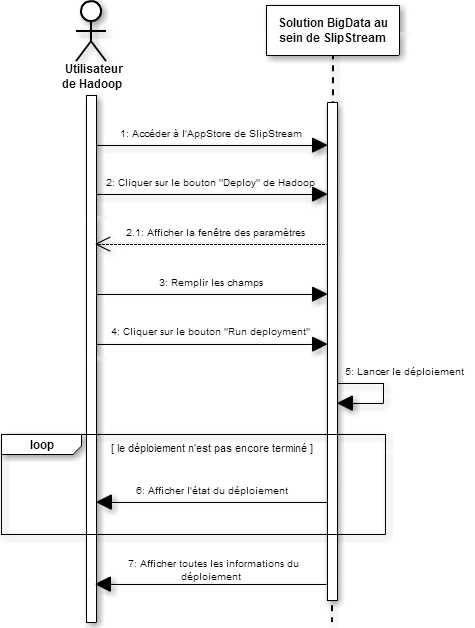
\includegraphics[scale=0.64]{Diagramme-deploy.png}
\caption{Digramme de s�quence de d�ploiement d'un cluster Hadoop}
\label{fig:fig3-2}
\end{figure}



\subsubsection{Cas d'utilisation 'G�rer les services de Hadoop'}
Une fois le cluster Hadoop d�ploy�, le syst�me affiche un lien pour que les utilisateurs acc�dent � l'outil d'administration en mode SaaS et s'authentifient en utilisant le couple (login et mot de passe) fourni par le syst�me. Par suite, ils g�rent et contr�lent tous les services via cet outil. Ce sc�nario est illustr� dans le diagramme de la figure \ref{fig:fig3-3} .
\begin{figure}[H]\centering
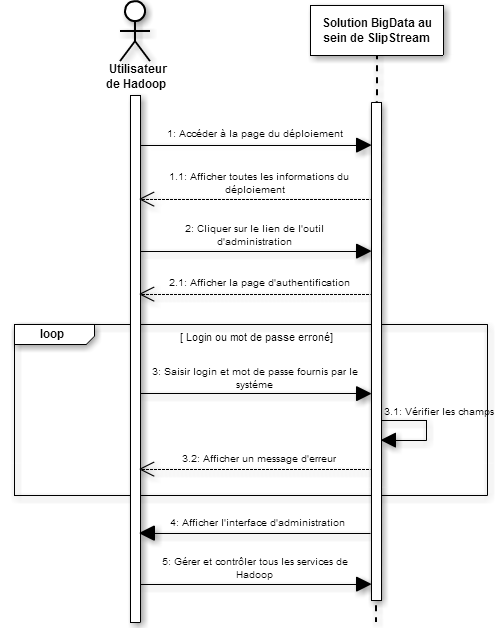
\includegraphics[scale=0.7]{Diagramme-Gerer.png}
\caption{Digramme de s�quence de gestion des services de Hadoop}
\label{fig:fig3-3}
\end{figure}


 
\section*{Conclusion}
Tout au long de ce chapitre, nous avons sp�cifi� et formul� les principales fonctionnalit�s que le syst�me con�u doit offrir. Par cons�quent. Nous r�pondons, ainsi, � ces besoins dans les �tapes suivantes en compl�tant l'�tude par les phases de conception et de mise en oeuvre du syst�me. Le chapitre suivant est consacr� � la conception de notre solution Big Data au sein de la plateforme SlipStream.





%==============================================================================
\end{spacing}


\backmatter
\pagestyle{fancy}
\fancyhf{}
\renewcommand{\chaptermark}[1]{\markboth{Conclusion G�n�rale et Perspectives}{}}
\fancyhead[R]{Conclusion G�n�rale et Perspectives}
\fancyfoot[R]{\thepage}
\renewcommand{\headrulewidth}{0.5pt}
\renewcommand{\footrulewidth}{0pt}
\chapter{Conclusion G�n�rale et Perspectives}
%==============================================================================
\pagestyle{fancy}
\fancyhf{}
\fancyhead[R]{\bfseries\rightmark}
\fancyfoot[R]{\thepage}
\renewcommand{\headrulewidth}{0.5pt}
\renewcommand{\footrulewidth}{0pt}
\renewcommand{\chaptermark}[1]{\markboth{\MakeUppercase{\chaptername~\thechapter. #1 }}{}}
\renewcommand{\sectionmark}[1]{\markright{\thechapter.\thesection~ #1}}

\begin{spacing}{1.2}
%==============================================================================

C'est l'une des parties les plus importantes et pourtant les plus n�glig�es 
du rapport. Ce qu'on \underline{ne veut pas voir} ici, c'est combien ce stage vous a �t� b�n�fique, comment il vous a appris � vous int�grer, � conna�tre le monde du travail, etc.\\
Franchement, personne n'en a rien � faire, du moins dans cette partie. Pour cela, vous 
avez les remerciements et les d�dicaces, vous pourrez vous y exprimer � souhait.\\
La conclusion, c'est tr�s simple : c'est d'abord le r�sum� de ce que vous avez racont�
dans le rapport : vous reprenez votre contribution, en y ajoutant ici les outils que vous 
avez utilis�, votre mani�re de proc�der. Vous pouvez m�me mettre les difficult�s
rencontr�es. En deuxi�me lieu, on y met les perspectives du travail : ce qu'on pourrait 
ajouter � votre application, comment on pourrait l'am�liorer.

%==============================================================================
\end{spacing}

\bibliographystyle{Biblio/unsrt_modif} 
\singlespacing
\renewcommand{\bibname}{Bibliographique}

\bibliography{Biblio/aesm_edspia}

\onehalfspacing

\appendix
\setcounter{figure}{0} 
\setcounter{table}{0}
\setcounter{footnote}{0}
\setcounter{equation}{0}
\pagestyle{fancy}
\fancyhf{}
\renewcommand{\chaptermark}[1]{\markboth{\MakeUppercase{#1 }}{}}
\renewcommand{\sectionmark}[1]{\markright{\thesection~ #1}}
\fancyhead[RO]{\bfseries\rightmark}
\fancyhead[LE]{\bfseries\leftmark}
\fancyfoot[RO]{\thepage}
\fancyfoot[LE]{\thepage}
\renewcommand{\headrulewidth}{0.5pt}
\renewcommand{\footrulewidth}{0pt}

\makeatletter
\renewcommand\thefigure{A.\arabic{figure}}
\renewcommand\thetable{A.\arabic{table}} 
\makeatother

\chapter{Annexe : Remarques Diverses}
\graphicspath{{Annexe1/figures/}}
%==========================================================================

%    Annexe

%===========================================================================
\begin{itemize}
\item Un rapport doit toujours �tre bien num�rot�;
\item De pr�f�rence, ne pas utiliser plus que deux couleurs, ni un caract�re fantaisiste; 
\item Essayer de toujours garder votre rapport sobre et professionnel; 
\item Ne jamais utiliser de je ni de on, mais toujours le nous (m�me si tu as tout fait tout seul); 
\item Si on n'a pas de paragraphe 1.2, ne pas mettre de 1.1;
\item TOUJOURS, TOUJOURS faire relire votre rapport � quelqu'un d'autre (de pr�f�rence qui n'est pas du domaine) pour vous corriger les fautes d'orthographe et de fran�ais;
\item Toujours valoriser votre travail : votre contribution doit �tre bien claire et mise en �vidence; 
\item Dans chaque chapitre, on doit trouver une introduction et une conclusion;
\item Ayez toujours un fil conducteur dans votre rapport. Il faut que le lecteur suive un raisonnement bien clair, et trouve la relation entre les diff�rentes parties;
\item Il faut toujours que les abr�viations soient d�finies au moins la premi�re fois o� elles sont utilis�es. Si vous en avez beaucoup, utilisez un glossaire.
\item Vous avez tendance, en d�crivant  l'environnement mat�riel, � parler de votre ordinateur, sur lequel vous avez d�velopp� : ceci est inutile. Dans cette partie, on ne cite que le mat�riel qui a une influence sur votre application. Que vous l'ayez d�velopp� sur Windows Vista ou sur Ubuntu n'a aucune importance;
\item Ne jamais mettre de titres en fin de page; 
\item Essayer toujours d'utiliser des termes fran�ais, et �viter l'anglicisme. Si certains termes  sont plus connus en  anglais, donner leur �quivalent en fran�ais la premi�re fois que vous les utilisez, puis utilisez le mot anglais, mais en italique;
\item �viter les phrases trop longues : clair et concis, c'est la r�gle g�n�rale !\\

\newpage

\textbf{Rappelez vous que votre rapport est le visage de votre travail : un mauvais rapport peut �clipser de l'excellent travail. Alors pr�tez-y l'attention n�cessaire.}

 
\begin{figure}[!ht]\centering

\includegraphics[scale=0.5]{ingenieur.jpg}
\end{figure}
\end{itemize}



\end{document}